\chapter{Практическая часть}

\section{Реализация}

В листингах~\ref{lst:unDens}-\ref{lst:unDist} представлена реализация функции плотности распределения и функции распределения вероятностей
случайной величины, распределенной по равномерному закону.

\begin{lstlisting}[label=lst:unDens, caption=Реализация функции плотности равномерного распределения]
private func uniformDensity(a: Double, b: Double, x: Double) -> Double {
    return (a <= x && x <= b) ? 1 / (b - a) : 0
}
\end{lstlisting}

\begin{lstlisting}[label=lst:unDist, caption=Реализация функции равномерного распределения]
private func uniformDistribution(a: Double, b: Double, x: Double) -> Double {
    if x < a { return 0 }
    if x > b { return 1 }
    
    return (x - a) / (b - a)
}
\end{lstlisting}

В листингах~\ref{lst:norDens}-\ref{lst:norDist} представлена реализация функции плотности распределения и функции распределения вероятностей
случайной величины, распределенной по нормальному закону.

\begin{lstlisting}[label=lst:norDens,caption=Реализация функции плотности нормального распределения]
private func normalDensity(mu: Double, sigma: Double, x: Double) -> Double {
    let pi = 3.14
    
    return 1 / (sigma * sqrt(2 * pi)) * exp(-pow(x - mu, 2) / (2 * sigma * sigma))
}
\end{lstlisting}

\begin{lstlisting}[label=lst:norDist, caption=Реализация функции нормального распределения]
private func normalDistribution(mu: Double, sigma: Double, x: Double) -> Double {
    return 0.5 * (1 + erf((x - mu) / (sigma * sqrt(2))))
}
\end{lstlisting}

\section{Примеры графиков}

На рисунках \ref{fig:uniform1} ---\ref{fig:uniform2} представлены графики функций равномерного распределения.

\begin{figure}[h!]
	\centering{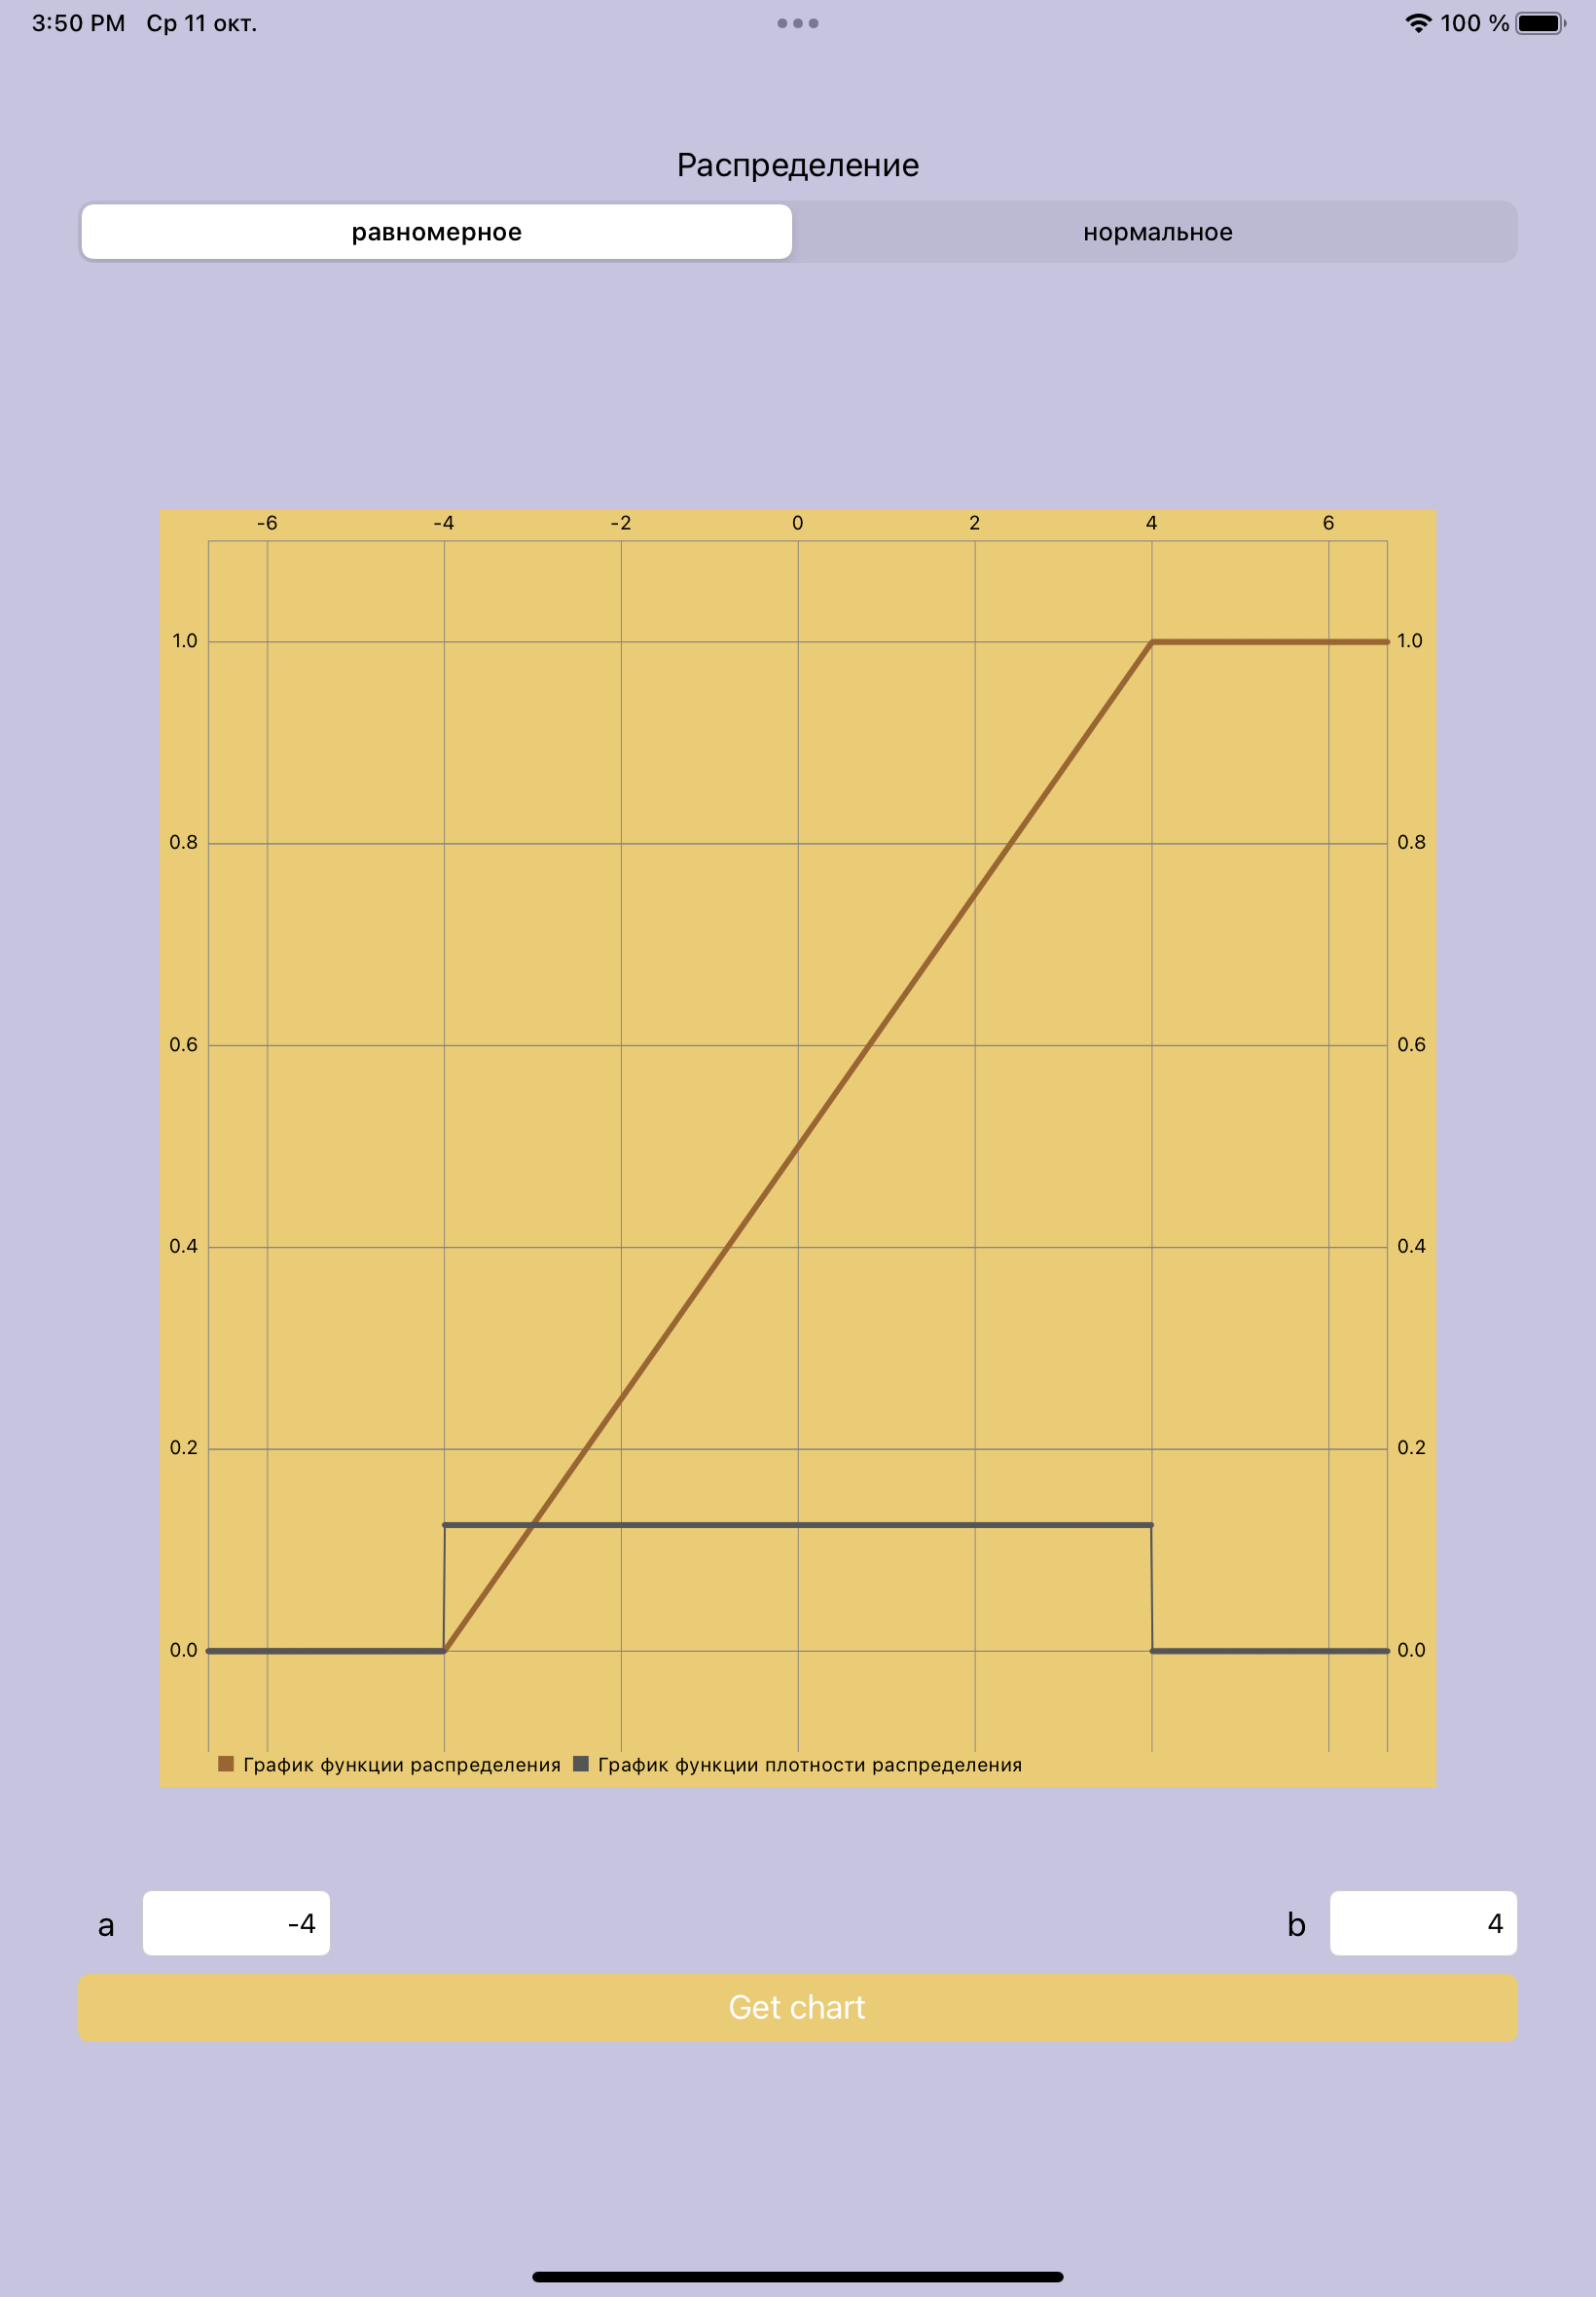
\includegraphics[scale=0.25]{img/uniform1.png}}
	\caption{Равномерное распределение при $a = -4$ и $b = 4$}
	\label{fig:uniform1}
\end{figure}

\begin{figure}[h!]
	\centering{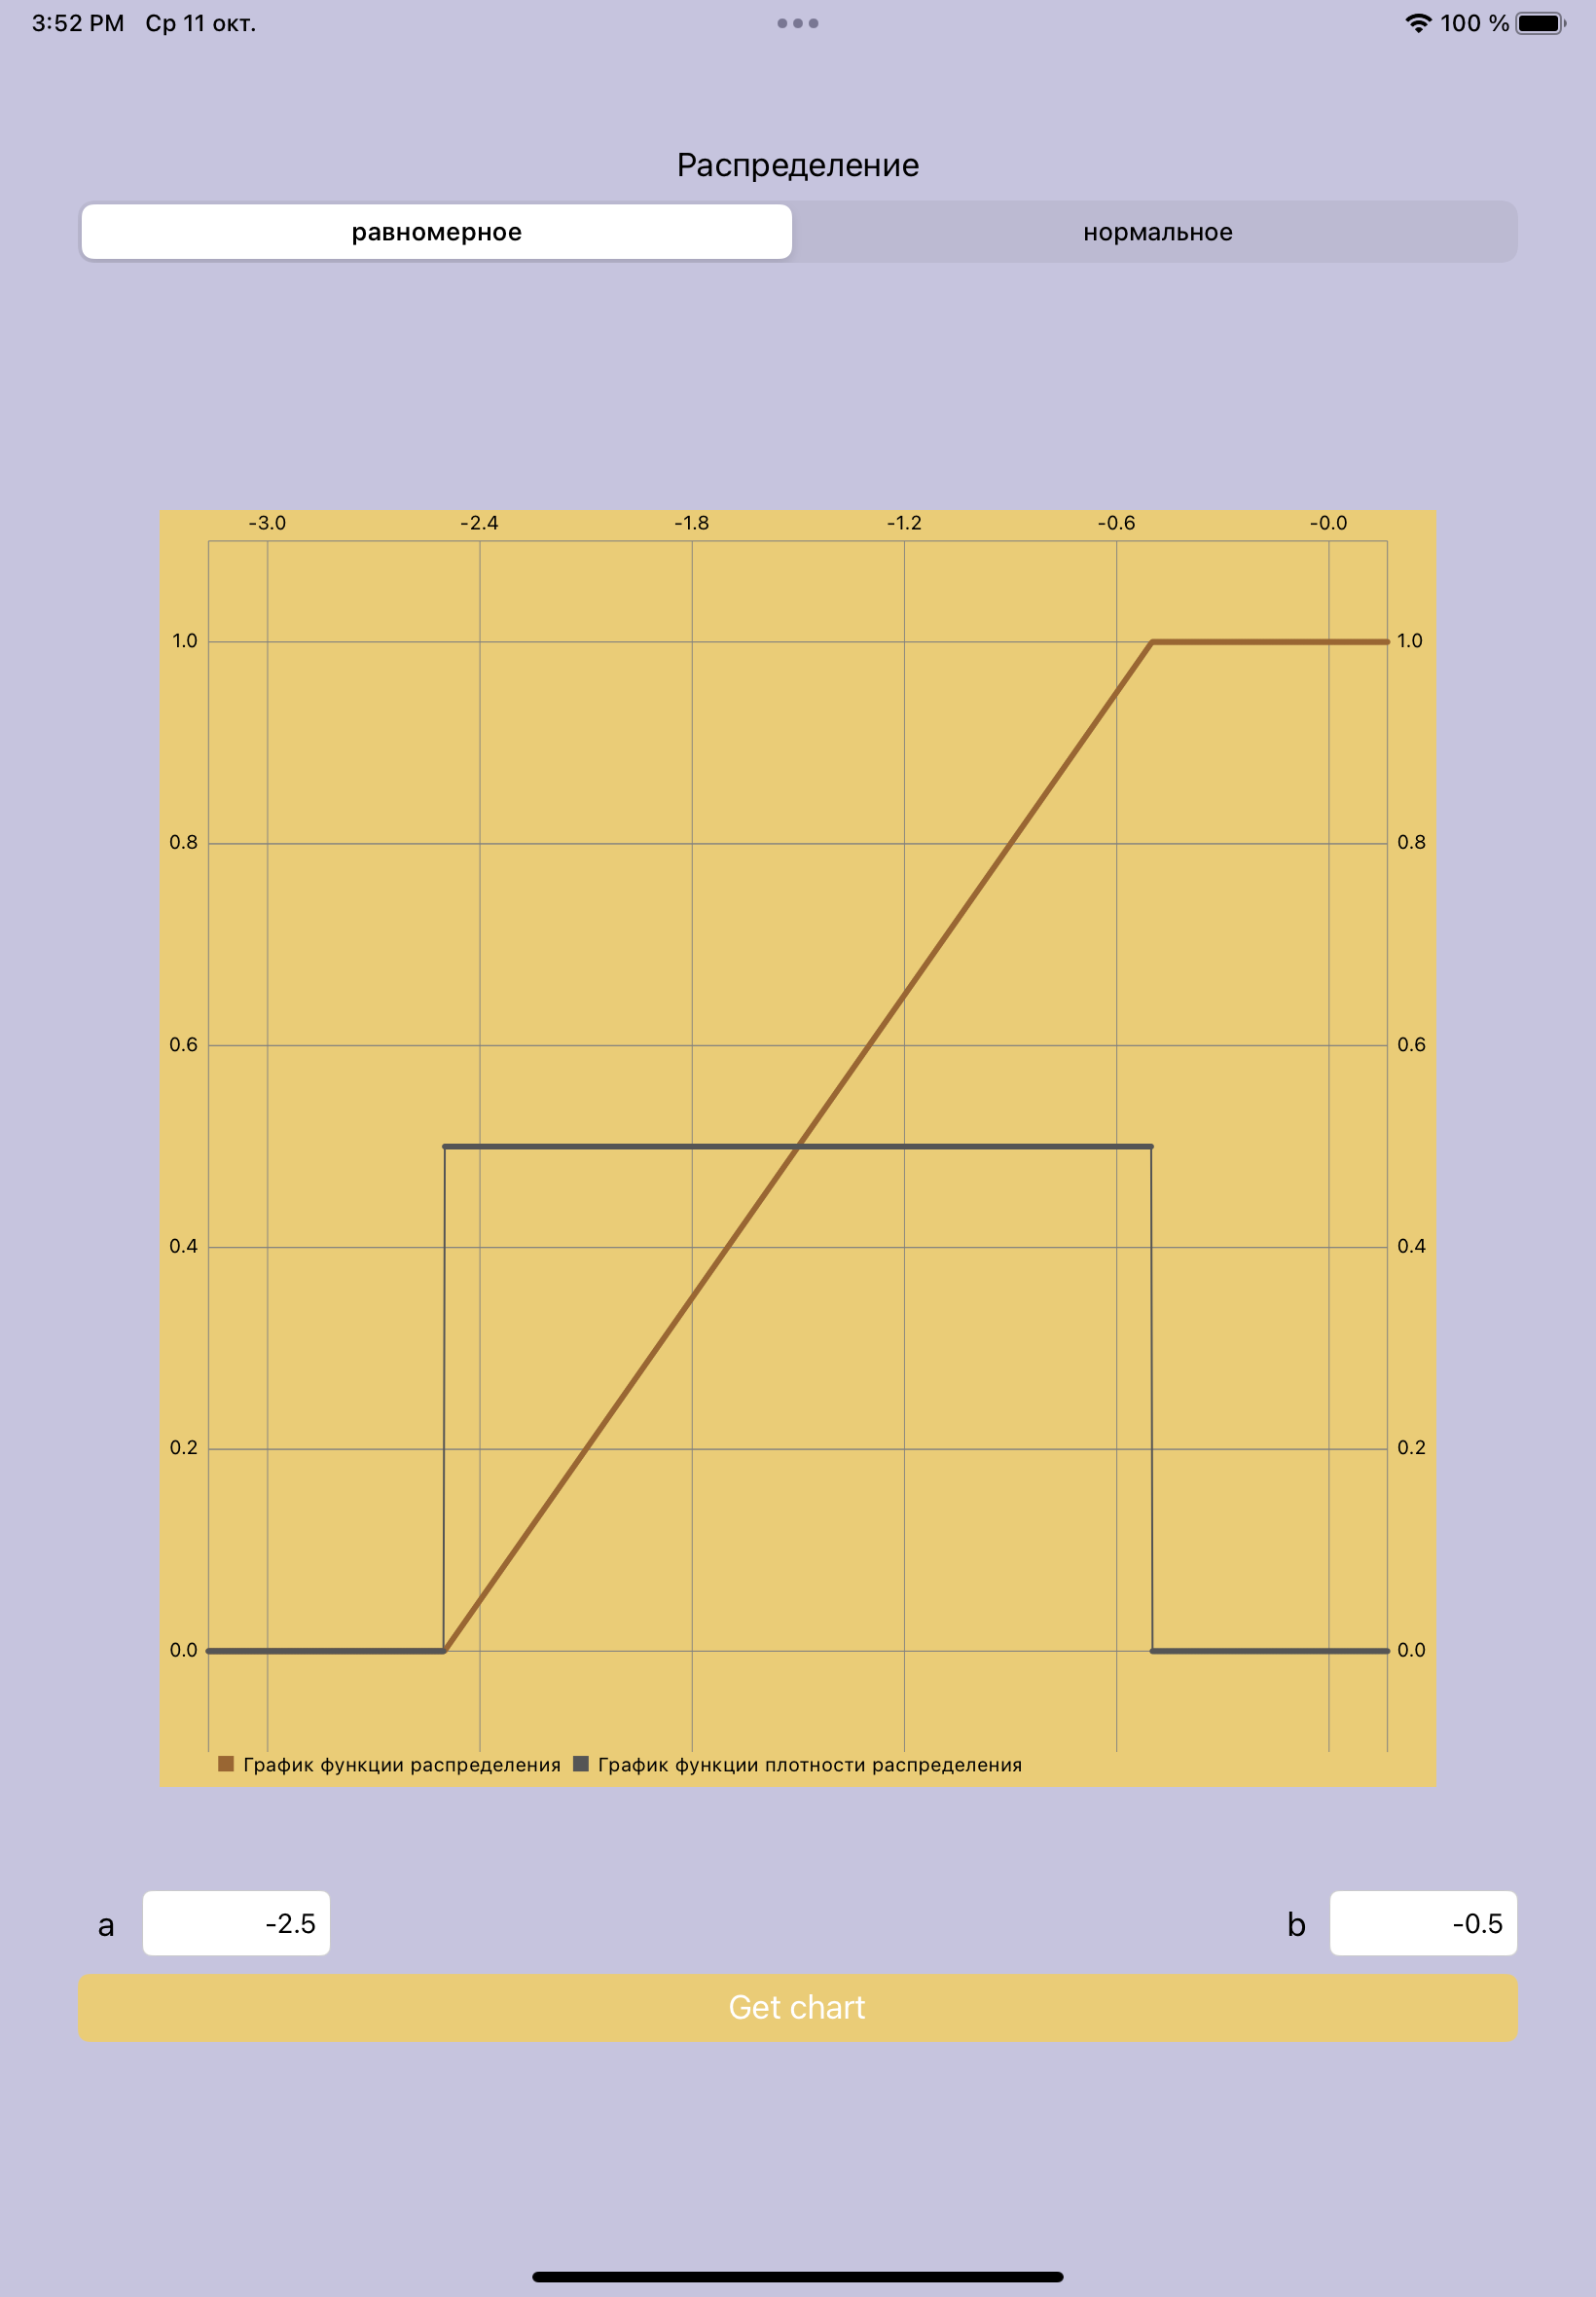
\includegraphics[scale=0.25]{img/uniform2.png}}
	\caption{Равномерное распределение при $a = -2.5$ и $b = -0.5$}
	\label{fig:uniform2}
\end{figure}

\newpage
На рисунках \ref{fig:normal1} ---\ref{fig:normal2} представлены графики функций нормального распределения.

\begin{figure}[h!]
	\centering{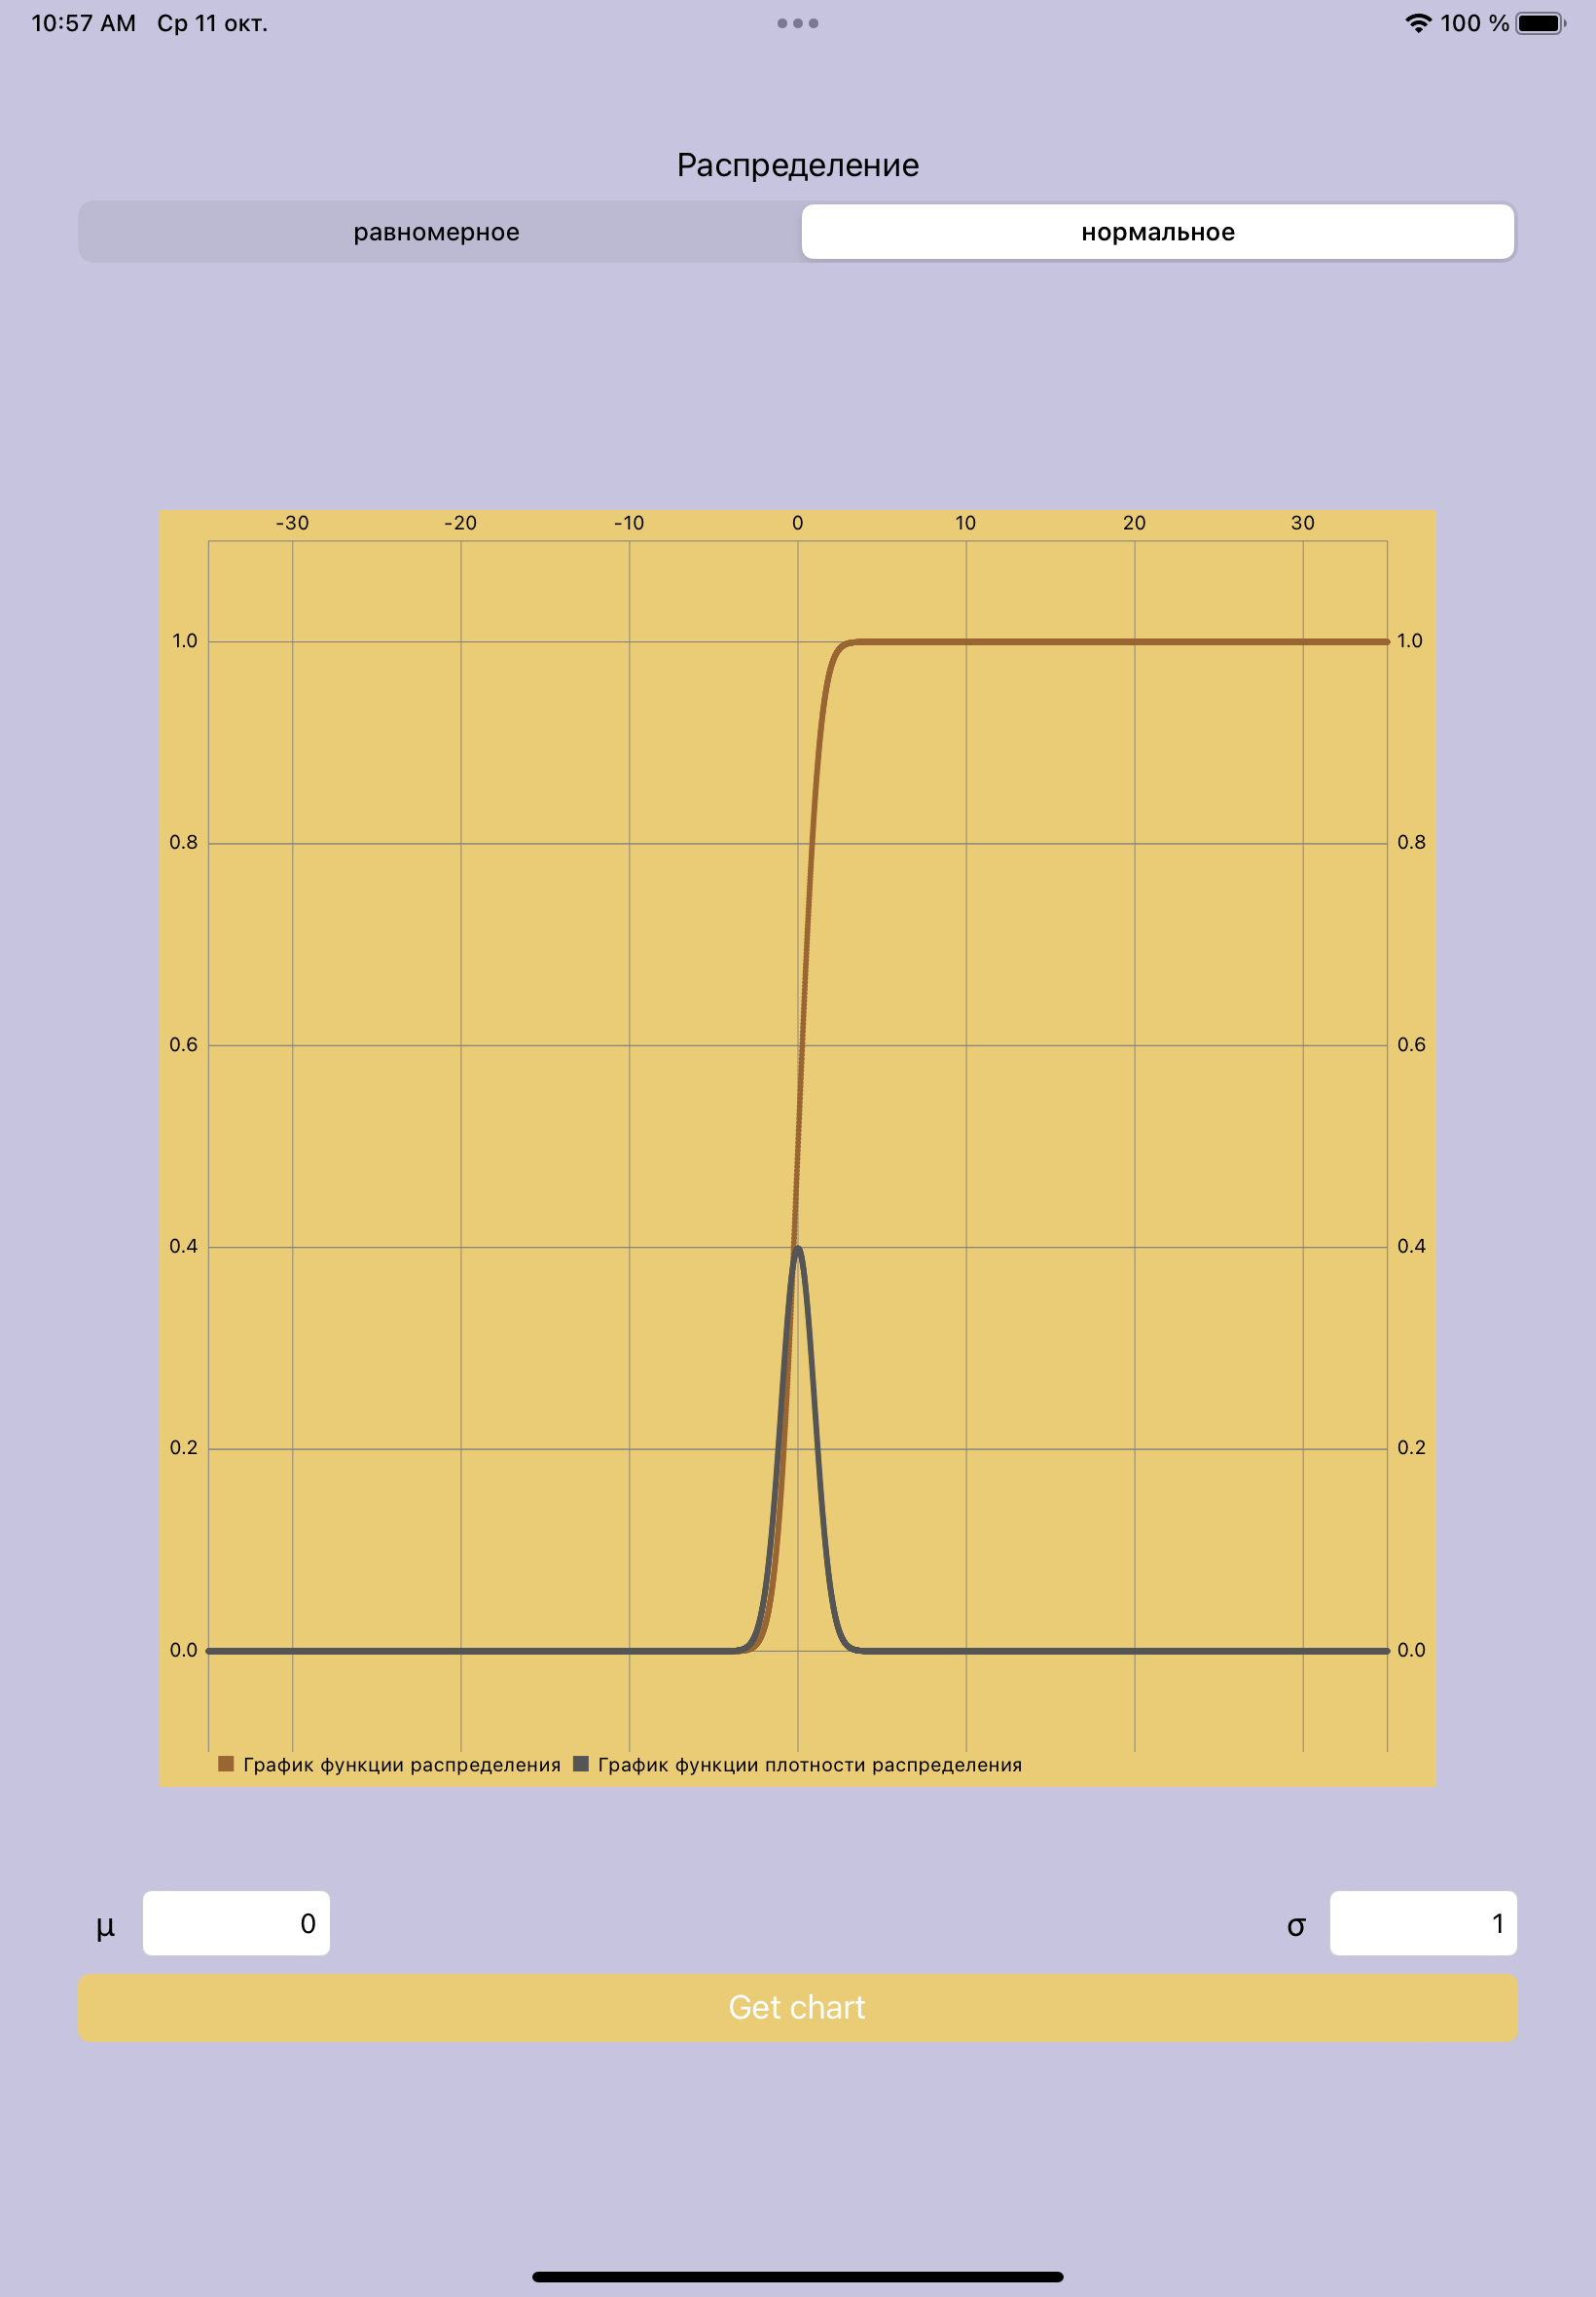
\includegraphics[scale=0.25]{img/normal1.png}}
	\caption{Нормальное распределение при $\mu = 0$ и $\sigma = 1$}
	\label{fig:normal1}
\end{figure}

\begin{figure}[h!]
	\centering{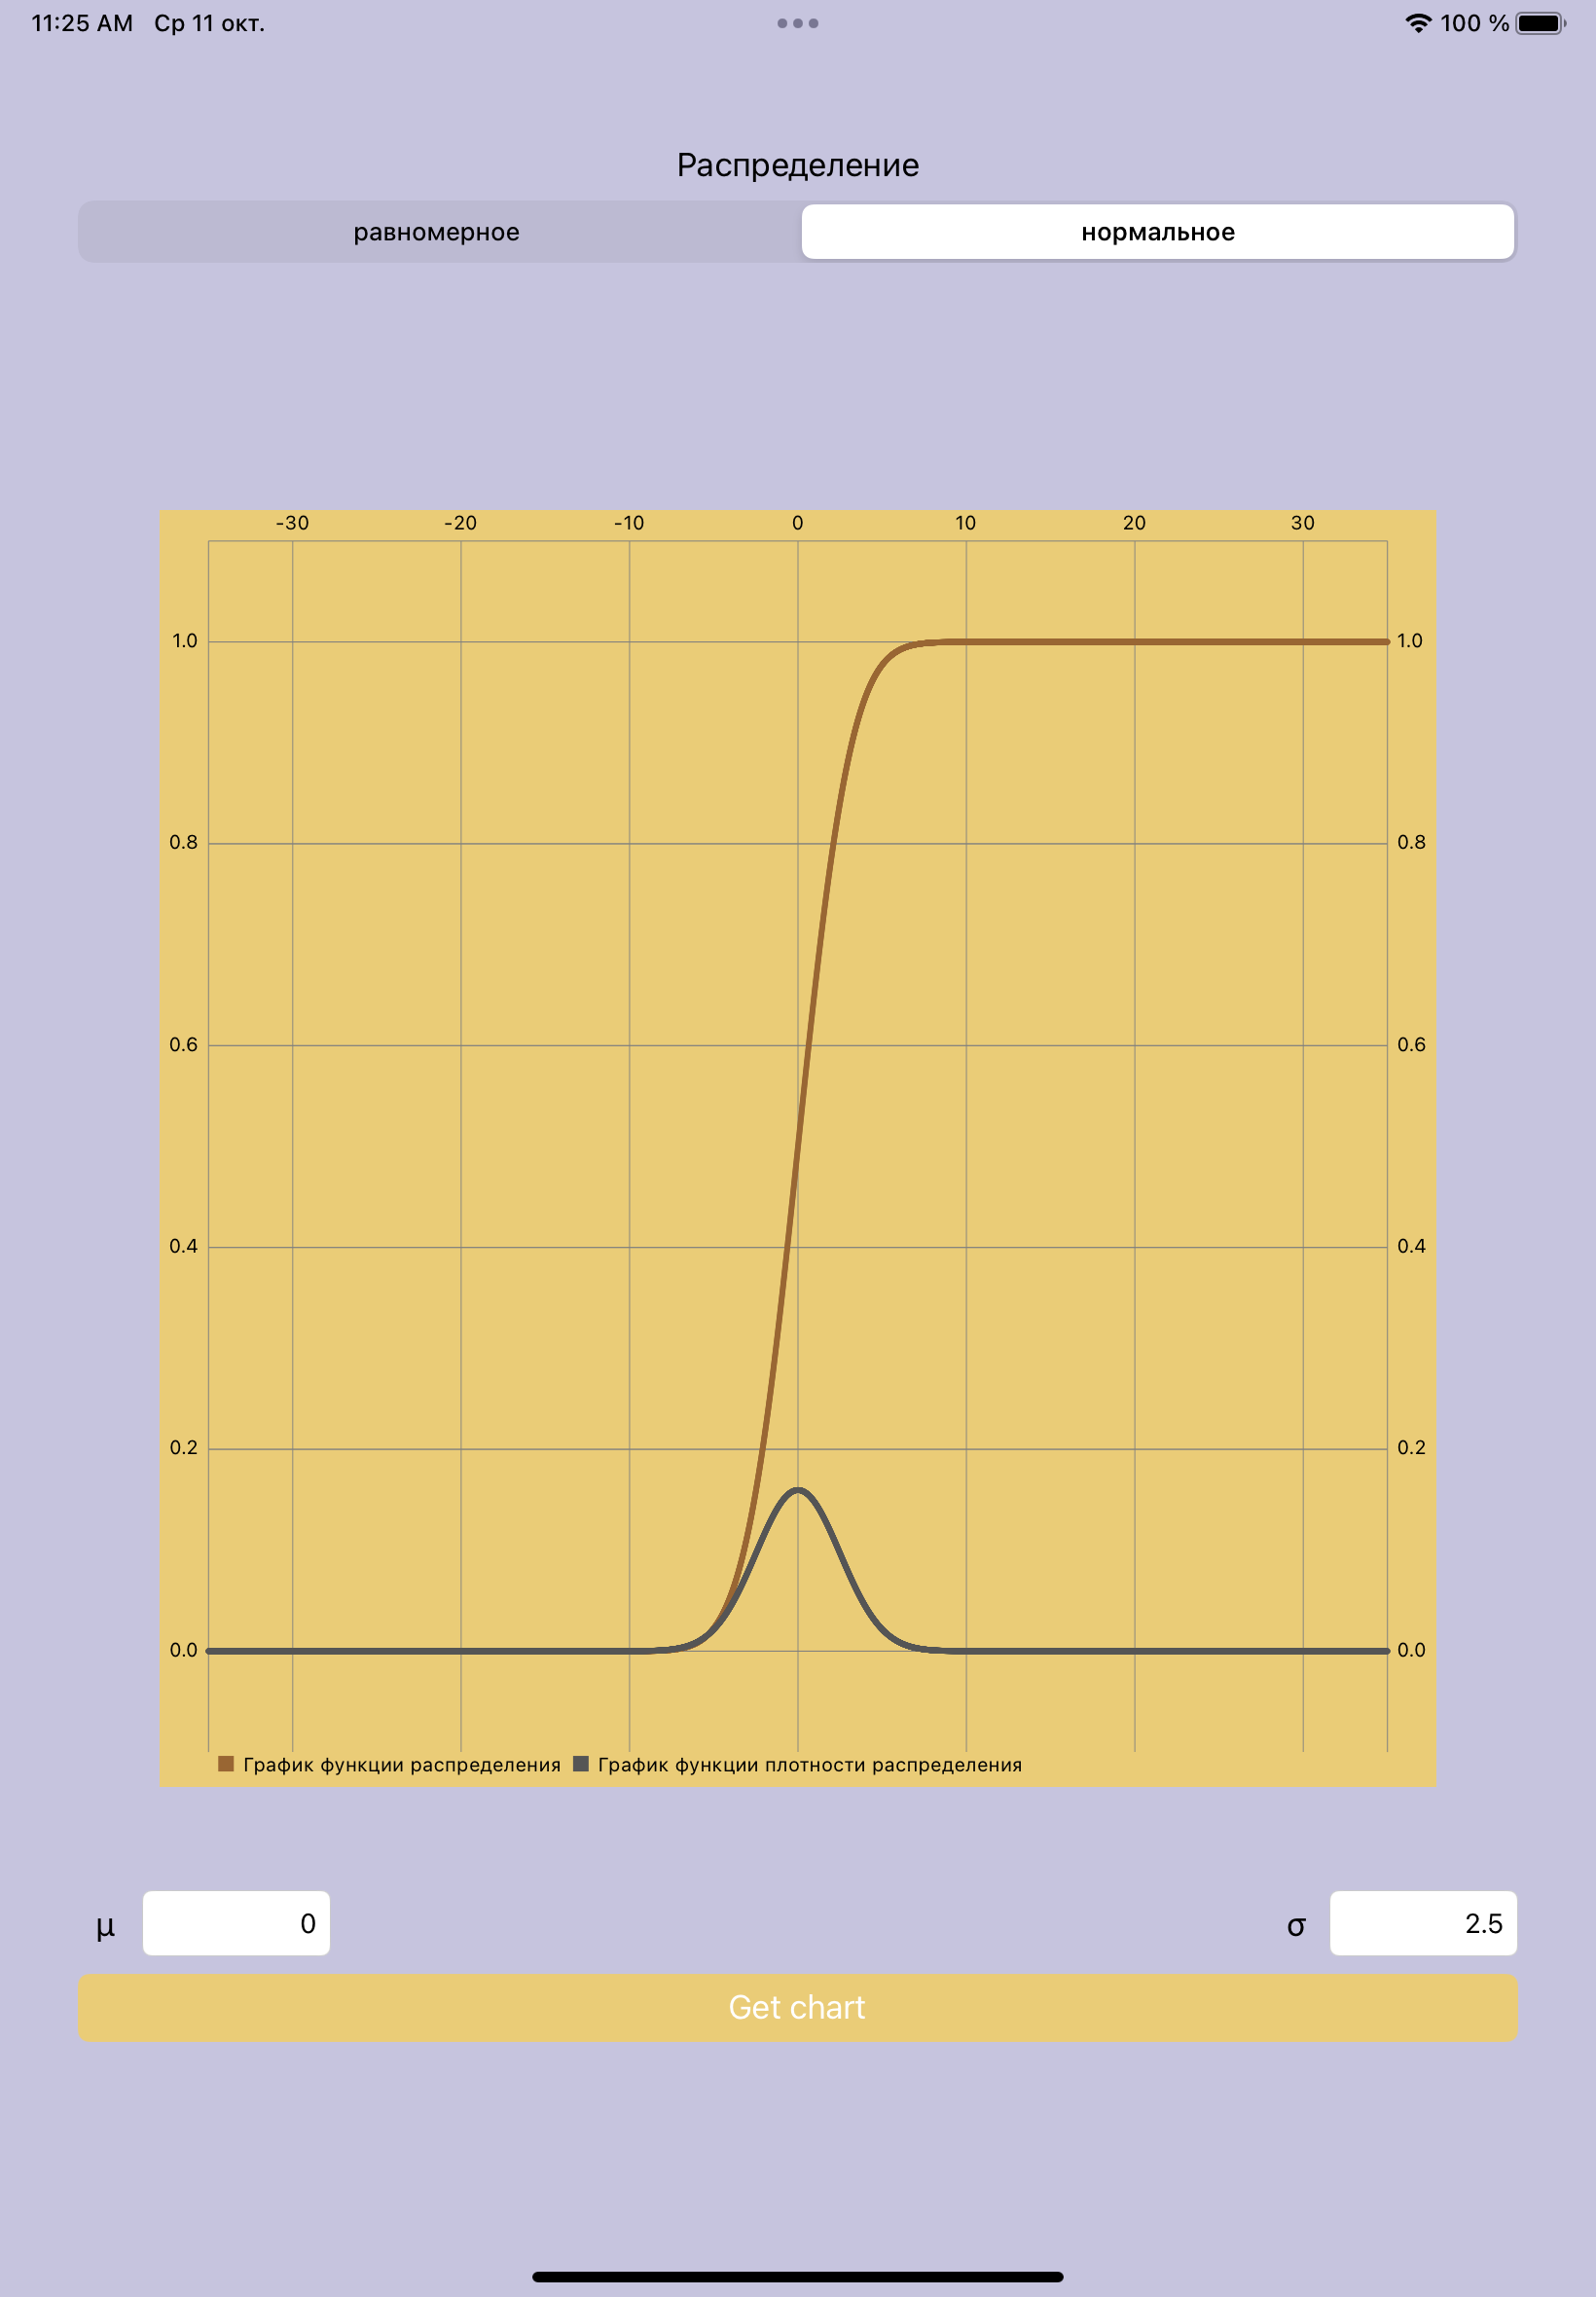
\includegraphics[scale=0.25]{img/normal2.png}}
	\caption{Нормальное распределение при $\mu = 0$ и $\sigma = 2.5$}
	\label{fig:normal2}
\end{figure}


